\documentclass[12pt]{article}
\usepackage{lmodern}
\usepackage{hyperref}
\usepackage{setspace}
\usepackage{float}
\hypersetup{
	colorlinks,
	citecolor=black,
	filecolor=black,
	linkcolor=black,
	urlcolor=black	
}
\usepackage{longtable}
\usepackage{amsmath}
\usepackage{listings}
\usepackage{graphicx}
\usepackage{subcaption} 
\usepackage{caption}
\usepackage{geometry}
\usepackage{enumerate}
\usepackage{array, booktabs}  
%\usepackage{multirow}
%\usepackage{tabularx}
\geometry{
	a4paper ,
	total={170mm,257mm},
	left=23mm,
	top=25mm,
	bottom = 25mm,
	right = 23mm
}	
\usepackage{fancyhdr}
\usepackage{gensymb}
\pagestyle{fancy}
\DeclareGraphicsExtensions{.jpg,.png,.pdf}

\usepackage{anyfontsize}

\lhead{}
\chead {ANLP Assignment 1}
\rhead{}
\cfoot{\thepage}

\usepackage[utf8]{inputenc}
\usepackage{color}

\definecolor{deepblue}{rgb}{0,0,0.5}
\definecolor{deepred}{rgb}{0.6,0,0}
\definecolor{deepgreen}{rgb}{0,0.5,0}
% Python style for highlighting


% Default fixed font does not support bold face
\DeclareFixedFont{\ttb}{T1}{txtt}{bx}{n}{12} % for bold
\DeclareFixedFont{\ttm}{T1}{txtt}{m}{n}{12}  % for normal

\newcommand\pythonstyle{\lstset{
		language=Python,
		basicstyle=\ttm,
		otherkeywords={self},             % Add keywords here
		keywordstyle=\ttb\color{deepgreen},
		emph={isEngAlpha,preprocess_line},          % Custom highlighting
		emphstyle=\ttb\color{deepblue},    % Custom highlighting style
		stringstyle=\color{deepred},
		frame=tb,                         % Any extra options here
		showstringspaces=false            % 
}}


% Python environment
\lstnewenvironment{python}[1][]
{
	\pythonstyle
	\lstset{#1}
}
{}


\usepackage{algorithm}
\usepackage[noend]{algpseudocode}

\makeatletter
\def\BState{\State\hskip-\ALG@thistlm}
\makeatother

\usepackage[nottoc,numbib]{tocbibind}


\setlength{\tabcolsep}{18pt}
\renewcommand{\arraystretch}{1.5}
% To Dos:
% Add comments to code - place comments on inputs/outputs of functions too apparently


\begin{document}	
	
\begin{titlepage}
	\newcommand{\HRule}{\rule{\linewidth}{0.5mm}} % Defines a new command for the horizontal lines, change thickness here
	\center % Center everything on the page
	\includegraphics[width = 0.3 \linewidth]{"./graphics/avatar-roundel-blackonwhite"}\\[0.5cm]
	\textsc{\\[1cm]\LARGE ACCELERATED NATURAL LANGUAGE \\
             \hfill\break PROCESSING}\\[2cm]

	\HRule \\[0.4cm]
	{ \huge \bfseries Assignment 1}\\[0.1cm]
	\HRule \\[1.5cm]
	\Large
	\vfill
	 S1818699, S1884908\\[0.5cm]
	{\large October 2018}
\end{titlepage}
\setlength\parindent{0pt}		
\newpage

\tableofcontents

\newpage
	
\section{Introduction}
The main scope of this assignment was to build trigram character models, and use them to produce random output or analyze text perplexity.  This report details the methodology followed to achieve these aims, and includes a discussion of the results obtained throughout the process.
\section{Preprocessing Input File - Question 1}
\subsection{Code}
The code in Listing \ref{pp} demonstrates the methodology used to preprocess input lines.
\begin{python}[caption = {Line Preprocessing},label = {pp}]
def isEngAlpha(character):
#checks if character is specifically english
	if (character >= 'a' and character <= 'z'):
		return True
	elif (character >= 'A' and character <= 'Z'):
		return True
	else:
		return False

def preprocess_line(line):
#Preprocessing of an input line
	character_list = list()
	for character in line:
		if (isEngAlpha(character)): #english checker
			character_list.append(character.lower()) 
		elif (character.isspace() or character == "."): 
			character_list.append(character) #keep ' ','.'
		elif (character.isdigit()):
			# convert digits {0-9} to 0
			character_list.append('0') 
	line = "".join(character_list).rstrip('\n') # remove newline  
	line = '#'+line+'#' #adds sentence start/end markers
	return line
\end{python}
\subsection{Additional Steps in Preprocessing}
Besides removing the illegal characters from each input line as per the specification, a `\#' character has been added to the beginning and ending of each line. This preprocessing step has been adopted in order to also gather trigrams using the beginning/ending (represented as `\#'s) of lines as input characters.  This way, information on sentence starts/ends is not lost.  Otherwise, the system would only have been able to begin estimating trigrams from the third character onwards, for every line.\\
\hfill\break
Additionally, the newline character `\textbackslash n' at the end of each line has also been removed, to allow for a smooth flow between lines when building n-gram models, without the need for catering for the extra `\textbackslash n'.
\subsection{Sample Input and Output}
A sample input/output pair from the preprocessing function is provided below:\\
\hfill\break
Sample Input: Reanudación del período de sesiones\\
Sample Output: \#reanudacin del perodo de sesiones\#
\section{Determining the Given Model's Estimation Method - Question 2} 
The language model probabilities file contains the trigram followed by the probability of the trigram conditioned on the occurrence of the first two characters in the trigram. To make an assessment of the kind of estimation method used, consider trigrams beginning with zz. 'zz' is chosen because in English there are seldom any words that have a zz followed by a character. Hence the the probabilities of such trigrams should be low and similar. On examining the trigram probabilities beginning with `zz', it is observed that all such trigrams have a probability of  
$3.333 * 10^{-2}$.\\
Assuming the model has been smoothed using add alpha method. The formula for add alpha smoothing is :
\begin{equation}
 \dfrac{{count(c_{1}\ c_{2}\ c_{3})} + \alpha} {\sum count(c_1\ c_2)+ \alpha * |V|} 
\end{equation}\\  
$(c_1,c_2,c_3)$ refer to the first, second and third characters respectively in the trigram and $|V|$ is the size of the vocabulary.\\
When the count ($(c_1,c_2,c_3)$) = 0 and count ($(c_1,c_2,)$) = 0, equation 1 reduces to:
\begin{equation}
\dfrac{1} {|V|} 
\end{equation}\\  
In this case $|V|$ = 30 because $|V|$ is the size of the character set $ \in \{  \space ,.,0,\#,a,b,c,d,e,f,g,h,i,\\k,l,m,n,o,p,q,r,s,t,u,v,w,x,y,z\}$, hence
\begin{equation}
\dfrac{1} {|V|}  = \dfrac{1} {30} = 3.33 * 10^{-2}
\end{equation}\\
Hence we can conclude that either add one or add alpha smoothing technique has been applies for the estimation. Consider another set of trigrams beginning with `zy' . We have $p(zy\space| zy) = p(zy. | zy)$ = $3 * 10^{-1}$ and all other trigrams beginning with `zy' have a probability of $1.429 * 10^{-2}$. For instance, assuming that the count of zya = 0, equation 1 reduces to  
\begin{equation}
\dfrac{ \alpha} {\sum count(zy)+ \alpha * 30} = 1.429 * 10^{-2}
\end{equation}\\
This equation has two unknowns  $\alpha$ and $\sum count(zy)$.
The count(zy ) or count(zy.) is not known. Hence we cannot exactly determine the value of $\alpha$ mathematically. However, we can conclude with certainty that  either add alpha or add one smoothing technique has been applied. The reason add one is also a possibility is due to the reason that when we replace the value of $\alpha$ with 1 the add alpha smoothing equation reduces to a add one smoothing equation.
\begin{equation}
 \dfrac{{count(c_{1}\ c_{2}\ c_{3})} + \alpha} {\sum count(c_1\ c_2)+ \alpha * |V|} = \dfrac{{count(c_{1}\ c_{2}\ c_{3})} + 1} {\sum count(c_1\ c_2)+ 1 * |V|}  = \dfrac{{count(c_{1}\ c_{2}\ c_{3})} + 1} {\sum count(c_1\ c_2)+  |V|}
\end{equation}\\  
\section{Trigram Character Language Model - Question 3}
\subsection{Method used to estimate the probabilities of the trigram}
1. Collected the trigram counts for each of the three character sequence in the training document. This was stored in a python dictionary called tri\_counts.\\
2. Collected the bigram counts for each of the two character sequence in the training document. This was stored in a python dictionary called bi\_counts.\\
3. The trigram probabilities were estimated by referencing the tri\_counts for each trigram $(c_1,c_2,c_3)$ and dividing it by the bi\_counts of the bigram beginning with the first two characters of the trigram$(c_1,c_2)$, where $c_1,c_2,c_3 \in \{ ,.,0,\#,a,b,c,d,e,f,g,h,i,k,l,m,n,o,p,q,\\r,s,t,u,v,w,x,y,z\}$\\
The equation used to estimate the trigram probabilities is stated in Equation 1:
\begin{equation}
P(trigram = c_{1}\ c_{2}\ c_{3}|c_{1}\ c_{2})= \dfrac{count(c_{1}\ c_{2}\ c_{3})}{count(c_1\ c_2)} 
\end{equation}\\
$c_1,c_2,c_3$  refer to the first, second and third character in the trigram sequence.\\
\subsection{Simplifying assumptions made}
We have extended our model to be able estimate the probabilities of unseen trigrams in the training set. For this we have implemented add one smoothing, add alpha smoothing and smoothing by interpolation. We ultimately decide to use the add one smoothing technique in our language model, because it provided the best results in terms of complexity and results.

\subsection{n-grams with two character history `ng'}
\subsubsection{Expectation}
It is expected that the summation of all the probabilities of n-grams with two character history `ng' will be equal to 1. This is because in a trigram starting with ng the next character has to be a character $\in \{ ,.,0,\#,a,b,c,d,e,f,g,h,i,k,l,m,n,o,p,q,r,s,t,u,v,w,x,y,z\}. $This is because the data set has been preprocessed to only have these characters. Hence, when we sum all the probabilities of trigrams beginning with 'ng' conditioned on the occurrence of 'ng', the summation is bound to equal 1.  \\
\subsubsection{Results}
The results are tabulated in Table 1.
\begin{center}
	
	\begin{longtable}{ | p{5em} | p{6.5em} | } 
	\caption{n-grams and their probability with the two-character history `ng'}\\ 
	
	\hline
	\centering \textbf{n-gram }& \textbf{Probability \space\space {\scriptsize (4 decimal places)}} \\ 
	\hline
	\centering ng  &  0.78742 \\ 
	\hline
	\centering ng.&   0.02642\\ 
	\hline
	
	\hline
	\centering ng0  &   0.00126\\
	\hline
	
	\hline
	\centering ng\#   &  0.00252\\
	\hline
	
	\hline
	\centering nga   &  0.00377\\
	\hline
	
	\hline
	\centering ngb   &  0.00126\\
	\hline
	
	\hline
	\centering ngc   &  0.00126\\
	\hline
	
	\hline
	\centering ngd   &  0.00503\\
	\hline
	
	
	\hline
	\centering nge   &  0.08553\\
	\hline
	
	\hline
	\centering ngf    & 0.00252\\
	\hline
	
	
	\hline
	\centering ngg   &  0.00126\\
	\hline
	
	
	\hline
	\centering ngh   &  0.00126\\
	\hline
	
	\hline
	\centering ngi    & 0.00252\\
	\hline
	
	\hline
	\centering ngj    & 0.00126\\
	\hline
	
	\hline
	\centering ngk   &  0.00126\\
	\hline
	
	\hline
	\centering ngl    & 0.00377\\
	\hline
	
	\hline
	\centering ngm  &   0.00126\\
	\hline
	
	
	\hline
	\centering ngn   &  0.00252\\
	\hline
	
	
	\hline
	\centering ngo   &  0.00751\\
	\hline
	
	
	\hline
	\centering ngp   &  0.00126\\
	\hline
	
	\hline
	\centering ngq   &  0.00126\\
	\hline
	
	\hline
	\centering ngr    & 0.01258\\
	\hline
	
	\hline
	\centering ngs   &  0.02138\\
	\hline
	
	\hline
	\centering ngt    & 0.01384\\
	\hline
	
	\hline
	\centering ngu    & 0.00377\\
	\hline
	
	
	\hline
	\centering ngv     & 0.00126\\
	\hline
	
	\hline
	\centering ngw    & 0.00126\\
	\hline
	
	
	\hline
	\centering ngx    & 0.00126\\
	\hline
	
	\hline
	\centering ngy    & 0.00126\\
	\hline
	
	\hline
	\centering ngz    & 0.00126\\
	\hline
	
	\hline
	\centering \textbf{Summation}   &  \textbf{1.0000}\\
	\hline
\end{longtable}
\end{center}

\subsubsection{Conclusion}
The results match the expectation because the summation of all the probabilities determined empirically as shown in Table 1, equals one. This is in-line with the theoretical expectation stated stated in section 4.3.1 

\section{Random Sequence Generation - Question 4}
Random generation from the the trigram model is a `raw' application of the model, where the model's probabilities are translated directly into text.  This output should represent the type of text the model is trained on, and will  take on the features represented within the model's training source.  This section provides a brief analysis of how random generation is carried out on the model, and discusses the differences between the outputs of the given model and the model estimated on the English training data.
\subsection{Random Generation Algorithm}
To actually generate the sequence, the model must select which character to output given the previous two character sequence (bigram).  The model contains the probability of each possible character which can come after the particular bigram.  Thus, the model simply needs to randomly sample from this distribution and output the result to produce the next character in the sequence.  To do this, a probability binning system as in Figure \ref{fig:randomgen} was put in place.
\begin{figure}[H]
	\centering
	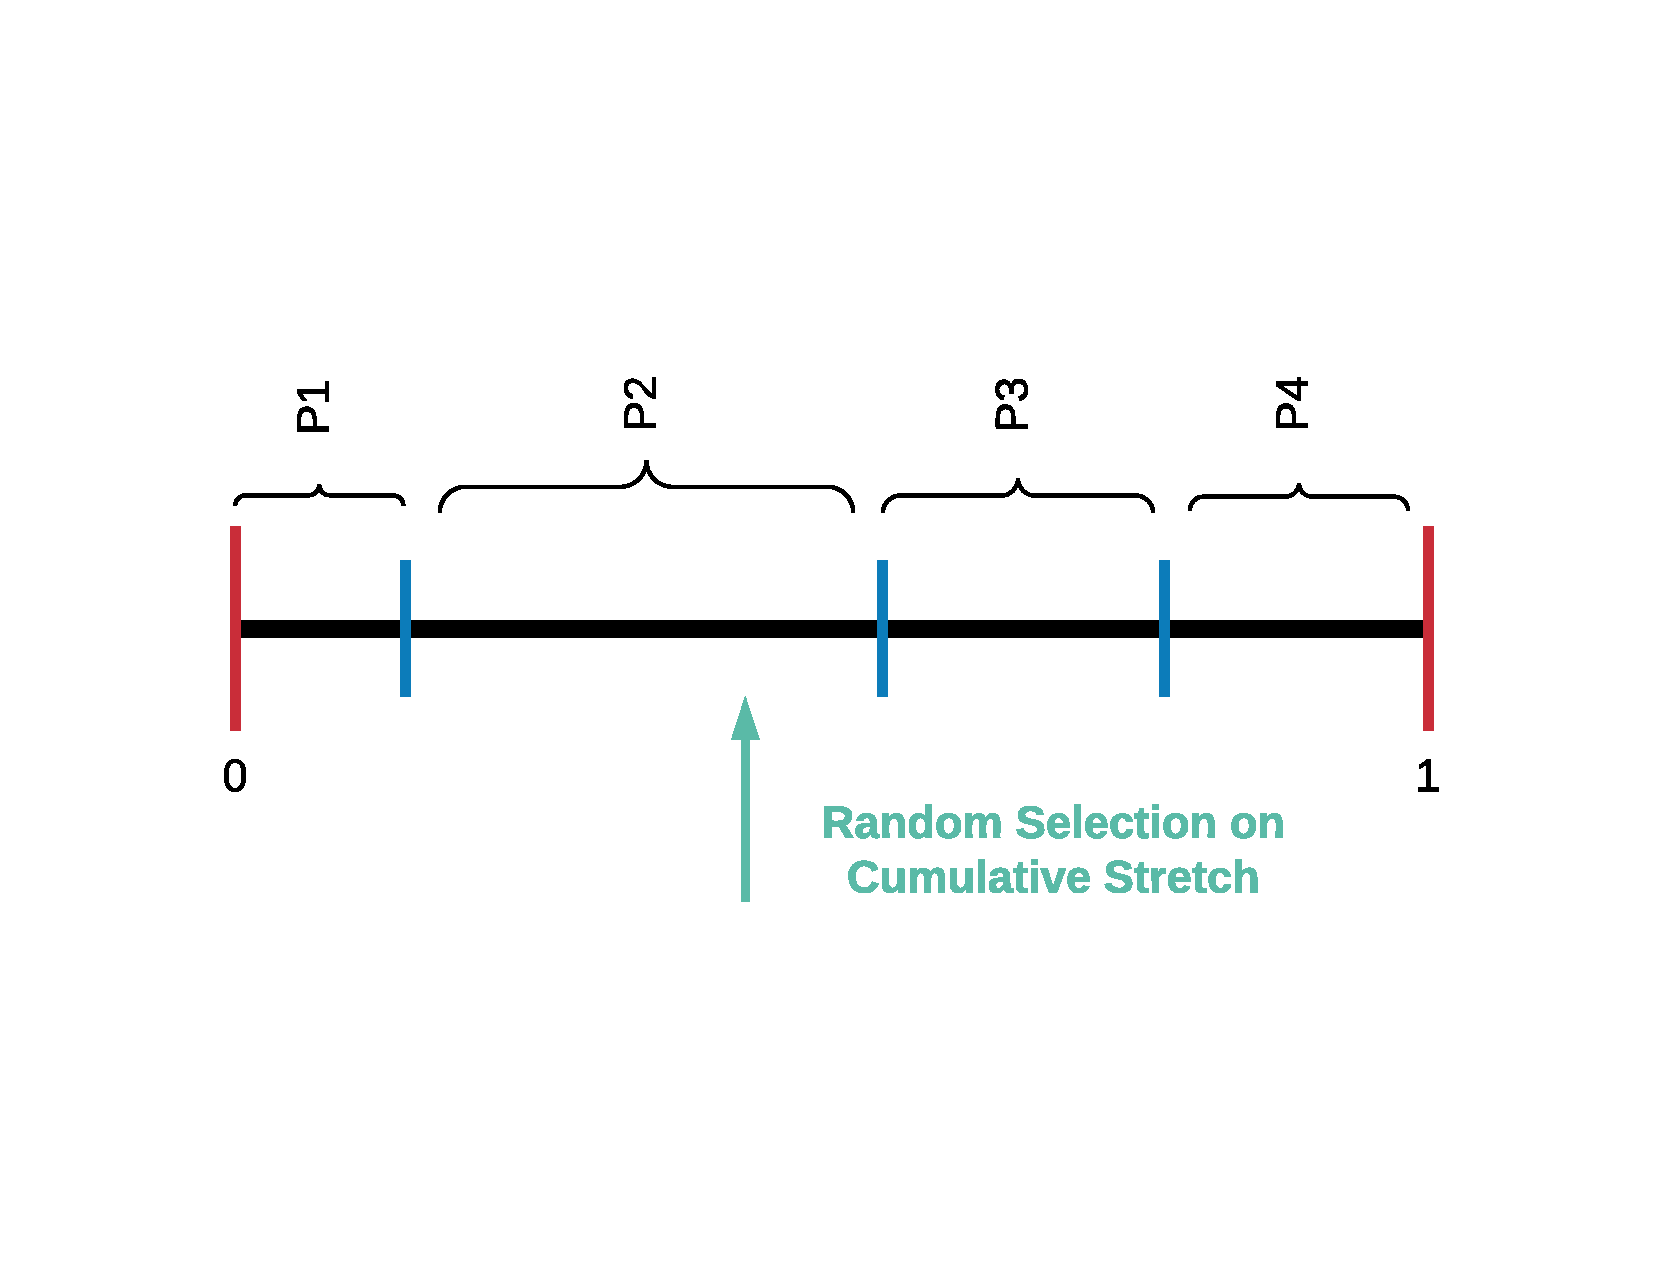
\includegraphics[width=0.7\linewidth]{graphics/Random_Gen}
	\caption{Random selection from a probability distribution}
	\label{fig:randomgen}
\end{figure}
Essentially, each probability in the distribution was put into bins corresponding to their size (as with P1,P2,P3 \& P4 in Figure \ref{fig:randomgen}).  With this setup in place, a random number was generated from the uniform continuous distribution, and the probability bin to which this number corresponded was selected as the next character in the sequence.  This system self-propagates itself; each new character produces a new bigram on which to base the next random generation.  The first bigram was set to always be a `\#' followed by a random character.\\
\hfill\break
Whenever a `\#' is generated, this signifies a line break (as explained in the answer to Question 1).  Thus, the system was set to automatically add another `\#' when this occurs, signifying both the end of a line and the start of a new one.  The next output character in the sequence will then be based on a `\#\#' bigram.  This system works for both the Europarl and given model.  The extra `\#' is of course not included in the count of random characters.\\
\hfill\break
The random generation process has also been summarised in pseudocode, as shown in \\Algorithm \ref{RanGen}.


\begin{algorithm}[H]
	\caption{Random Generation}\label{RanGen}
	\begin{algorithmic}[1]
		\Procedure{generate\_from\_lm}{Num\_Chars, Model, Valid\_Char\_List}
		\State $sequence = []$
		\State $bigram\_in \gets  \text{`\#'} + random(Valid\_Char\_List)$
		\State $chars\_left \gets Num\_Chars -1$
		\BState \emph{loop}:
		\If {$chars\_left > 0$}
				\If {$bigram\_in[1] == \text{`\#'} \ and\  bigram\_in[0]\ !=  \text{`\#'} $}
				\State $sequence \gets sequence +  \text{`\#'} $
				\Else
				\If {$bigram\_in == \text{`\#\#'}  $}
						    \State $possible\_tris \gets [bigram\_in + Valid\_Char\_List[excluding\ \text{`\#'}]]$.
				\Else
						     \State $possible\_tris \gets [bigram\_in + Valid\_Char\_List]$.
				\EndIf
		     	\State $distribution \gets model[possible\_tris]$.
		     	\State $bins \gets cumulative\_sum(distribution)$
		     	\State $distribution\_pos \gets random\_bin\_select(bins)$
		     	\State $new\_sequence \gets pos\_tris[distribution\_pos]$
		     	\State $bigram\_in \gets new\_sequence[0:1]$
		     	\State $sequence \gets sequence + new\_sequence[2]$
		     	\State $chars\_left \gets chars\_left - 1$
		     	\EndIf
		     	\State \textbf{goto} \emph{loop}.
				
		\EndIf
		\State \textbf{return} $sequence$
		\EndProcedure
	\end{algorithmic}
\end{algorithm}


\subsection{Sample Outputs}
When generating 300 sample characters of output from both models, two sample outputs obtained are shown below (\textcolor{red}{NL} signifies a new line, all `\#'s have been removed):\\

Generated from the Add-One-Smoothing Model trained on `training.en':\\
\hfill\break
\textit{.wyouterentlsol popmple be opmum pareen willon wity.\textcolor{red}{NL}\\
	mfte stragnu\textcolor{red}{NL}\\
	th thesion an lk.ltqnqake shou hatin actiong the we mad onlaticlasted betterevicand theqqltese the tooving miss ted\textcolor{red}{NL}\\
	welv0comh.x.gfunalwcnme counat implound thinitate trat to shose und be cof wo st pe of goin inagend thas new orwgoodur\\}
\hfill\break
Generated from the given model, `model-br.en':\\
\hfill\break
\textit{me it you ch ons.\textcolor{red}{NL}\\
	the get doggir.\textcolor{red}{NL}\\
	mor hose.\textcolor{red}{NL}\\
	whaskis it.\textcolor{red}{NL}\\
	ok.\textcolor{red}{NL}\\
	theres so thes doings.\textcolor{red}{NL}\\
	okay.\textcolor{red}{NL}\\
	what thet doin.\textcolor{red}{NL}\\
	them sho some right.\textcolor{red}{NL}\\
	oks.\textcolor{red}{NL}\\
	he ill one.\textcolor{red}{NL}\\
	wast wally not put want there buchats.\textcolor{red}{NL}\\
	ye.\textcolor{red}{NL}\\
	righ thesnt.\textcolor{red}{NL}\\
	hos tope.\textcolor{red}{NL}\\
	his dog.\textcolor{red}{NL}\\
	im his truseen ther.\textcolor{red}{NL}\\
	low yout apeer a toor.\textcolor{red}{NL}\\
	yeah.\textcolor{red}{NL}\\
	spee to tin you dog this backlif}
\subsection{Comments}
\begin{itemize}
	\item  The given model has line breaks after nearly every full stop.  The trained model places line breaks after full stops much less.  This  is possibly caused by the small size of the test data used.  The Europarl model has not prioritized new lines after full stops enough, even though most line breaks come after full stops in the training data. 
	\item  The given model produces much more new lines than the trained model.  The Europarl model has been trained on a corpus containing many long sentences, which explains why its output contains many long sentences in turn.  For the given model, this could possibly signify the model was training on data from some poem or text containing many short sentences.
	\item The given model actually produces some coherent words, whilst the Europarl model produces many more jumbled up words.  Again, this could be a consequence of the small size of the data used.  Interestingly, the given model contains many words such as `toy', `dog', `pup', `boy' or `daddy'.  This again points to the training text for this model being based on some kid-friendly text, possibly with very few sentences to make reading easier.  Of course, this could also be some form of dialogue between a child and his parents.  The Europarl model occasionally produces words such as `important' which appear frequently within the text.
\end{itemize}
\section{Perplexity Computation - Question 5}
Perplexity is a measure of how well a model can predict the characters within a text corpus.  Essentially, it shows how well a text file's contents are related to the probabilities stored within a model.  This section provides an analysis of the different languages model, and how it fares against familiar and unfamiliar types of inputs.
\subsection{Perplexity Computation}
The general equation for perplexity ($PP_{M}$) computation is shown in Equation \ref{PP}.
\begin{equation}\label{PP}
	PP_{M} = P_{M}\left( c_{1}.... c_{n}\right)^{-\frac{1}{n}}
\end{equation}
Where $P_{M}(...)$ is the product of the probability of each character($c_{i}$) in an input text, and $n$ is the total number of characters in the input.  Using direct probabilities, however, will result in a number which is too small for  proper representation.  Thus, a log system was used by converting the perplexity measure into a log perplexity measure as follows:
\[log\left(PP_{M}\right) = log\left(P_{M}\left( c_{1}.... c_{n}\right)^{-\frac{1}{n}}\right)\]

\[log\left(PP_{M}\right) = -\frac{1}{n}\times log\left(P_{M}\left( c_{1}.... c_{n}\right)\right)\]
\begin{equation}\label{logPP}
log\left(PP_{M}\right) = -\frac{1}{n} \sum_{i=1} ^{n}\left( log(P_{M}(c_{1})) + ... + log(P_{M}(c_{n})) \right)
\end{equation}
The result, Equation \ref{logPP}, can be easily converted back to the normal perplexity measure by taking the antilog of its value.  This system allows one to compute the perplexity without running into any numerical representation issues.  This system was implemented as a standalone function, along with a number of checks to deal with the double `\#' preprocessing and other inadmissible conditions.  
\subsection{Testing the Language Models}
The test document provided acts as being an `unseen' document, and should act as a good validation of the expected result for each language model, at least with an English text input.  Each language model with Add-One Smoothing was used to calculate the perplexity of the test document, with the results shown in Table \ref{TR} (the model file result has been added for comparison).
	\begin{table}[H]
	\centering
	\setlength\arrayrulewidth{1pt}
	\caption{\label{TR}Perplexity results on the English test file }
	\begin{tabular}{c  c }
		\hline
		\textbf{Language Model} & \textbf{Perplexity (4 decimal places)} \\
		\hline                     
	English& \textbf{8.8696}\\
	German & 22.9270 \\
	Spanish & 22.5249 \\
	Given & 22.0930\\
	\end{tabular}
\end{table}
Looking at these results, it is clear that from the three language models, the English model has found the test document to be the least perplex, and by a large margin ($\sim$13.5).  This should mean that, by analyzing a document with all three of the models, one should be able to easily infer the language of the test document by finding the outlier (and much lower) perplexity value.  Further perplexity tests were carried out on a Spanish \cite{GSpan} and German document \cite{GSpan}, the results of which are shown in Table \ref{SR}.

\begin{table}[H]
	\centering
	\setlength\arrayrulewidth{1pt}
	\caption{\label{SR}Perplexity results on Spanish and German test files }
	\begin{tabular}{c c c}
		\hline
		\textbf{Language Model} & \multicolumn{2}{c}{\textbf{Perplexity (4 decimal places)} }\\
		\hline
		  & \textbf{Spanish File} & \textbf{German File} \\
		\hline                     
		English& 22.6965 & 20.6750\\
		German & 29.3398 & \textbf{8.6951}\\
		Spanish & \textbf{11.3395} & 27.9311\\
		Given & 51.9747& 45.1458\\
	\end{tabular}
\end{table}

Again, the perplexity results show a clear indication towards the correct document language, with the margin of perplexity difference between the correct language and other languages being at least 11. 

\subsection{Document Language Determination}

Whilst using all three models in tandem results in a good language classifier, using just one model for classification does not, even just for detecting the model's trained language.  This is easy to confirm using just the two English models - the given model and the Europarl English model.\\
\hfill\break
Looking back at tables \ref{TR} and \ref{SR}, the given and Europarl model perplexity results vary considerably.  In Table \ref{TR}, the Europarl model reports back a perplexity of $\sim$8 whilst the given model reports a perplexity of $\sim$22.  Taking the Europarl model itself, one might think that it should be obvious that the test document is written in English.  However, had one used just the given model, one would think twice before deciding on the language!  It is entirely possible that the Europarl model could assign such a high perplexity to an English document too, if the document is written in a format very different (e.g. with very short sentences or with many slang words) to the one it was trained on.\\
\hfill\break
It is clear that using just one model in isolation is not enough to determine the language of a document.  One would need models of all the other possible languages the document could be in, in order to correctly deduce the document language.  Furthermore, each language model should ideally be trained on the same style and format of corpus (or a translation of the same corpus) in order to make sure that the only difference between models is in the language, and not in formatting or context.  
\subsection{Effects of Smoothing on Perplexity}
Two other methods of smoothing were implemented - Add Alpha Smoothing and Interpolation Smoothing.
% Add data here - should be insignificant
\section{Identifying Document Type - Question 6}

\section{Conclusions}
\begin{thebibliography}{2}
	\bibitem{FSpan}  Friends Script Spanish Translations: https://www.friendspeich.com/guiones01.php
\bibitem{GSpan}German Text Source: https://lingua.com/german/reading/
\end{thebibliography}

\end{document}
